\documentclass{article}
\usepackage{graphicx}

\begin{document}

\title{Team Meeting Summaries}
\author{Christian Plourde 26572499\\*
		Ayush Kharade 40042388\\*
		Daniel Vellucci 27416288\\*
		Samer Yazbeck 40049573\\*
		Luciano Porchet 40048537
		}
\date{Last Updated December 1st, 2019}

\maketitle

\newpage

\section{Meeting of September 18th, 2019}

\subsection{Meeting Duration}
75 Minutes

\subsection{Notes}
\subsubsection{Game Details}
\begin{description}
\item 3D characters, Platformer in a 2D view
\item Platformer
\item Singleplayer
\item Similar to Trine or This War of Mine
\item Genre: Action / Adventure platformer
\end{description}

\subsubsection{Story}
\begin{description}
\item Starts with “Hey you're finally awake!”\\*(wake up in a cave? Forest?, need a setting)
\item The Lord Ruler is dead, Ruin has been released.
\item Ruin is trying to destroy the world and has gained control of minions and people who become the enemies
\item Main character is fighting for survival and ends up destroying ruin in the end (or a higher level minion control directly by Ruin), so ruin is still out there, the possibility for a sequel.
\item Main character doesn't want to save the world but gets forced into doing it (joke story) 
\end{description}

\subsubsection{Enemies}
\begin{description}
\item Mistings (people who can burn one metal)
\item Koloss (large enemies that wield swords)
\item Coinshots(ranged?)
\item Regular minions (people under Ruin’s Control)
\end{description}

\subsubsection{Mistborn Mechanics}
\begin{description}
\item Burning metals (magic system called allomancy)
\item Iron - pull metal objects toward you
\item Steel - push metal objects away from you
\item Brass - Sooth people's emotions (could be used to make people fall asleep) (throwable?)
\item Zinc - Riot people's emotions (could be used to charm enemies to fight for you) (throwable?)
\item Tin - Heightens senses (could be used to see enemies past the fog of war)
\item Pewter - Makes user stronger, more agile, increases endurance and healing
\item Bronze - Detect another person burning metals (made from copper and tin)
\item Copper - Hide your metal burning from other people
\item Gold - See yourself in the past (is it implementable?)
\item Atium - see another person a few moments in the future (is it implementable?)
\item Collect metals from the environment
\item Hidden metals, scavenging
\item Crafted metals
\item Progression in usability of metal (start with a few, unlock more as you progress)
\item NPC to provide metals for you (buyable from shops)
\item Combining metals for different effects? (Could have it so you can't get steel without combining iron and carbon) (or iron and carbon do two different things but when combined they make objects static, this could be used for stasis puzzle mechanics)
\item Fog of war idea (light coming from player), only things that are illuminated can be affected by allomancy, or faint light coming from every character
\item Small puzzles to find rare metals
\item Ruin can change words (give fake hints to the player) player gambles if it is worth going there (could have traps or very powerful enemies in these areas)
\item Collect carbon from everywhere, if you don't use it all game it turns into diamond and you get an ultimate ability
\end{description}

\subsubsection{Combining Metals Mechanic}
\begin{description}
\item Alchemy table to combine metals or unlockable \& portable mortar and pestle (need to be out of combat or at a save point to combine metals)
\item Skill tree could be accessed from here too (requires to unlock skill to combine metals)
\end{description}

\subsubsection{Mistborn Setting}
\begin{description}
\item Black world, falling ash, red sun
\item Misty Environment
\item Mistcloaks
\end{description}

\subsubsection{Combat}
\begin{description}
\item Steel, iron fighting moving metal objects
\item Melee only available when you burn pewter
\end{description}

\subsubsection{Enemy Mechanics}
\begin{description}
\item Only attack if close enough, move towards you until it is close enough
\item Chase you to the end of the room then go back
\end{description}

\subsubsection{Supporting Art}
  \begin{figure}[!htb]
    \center{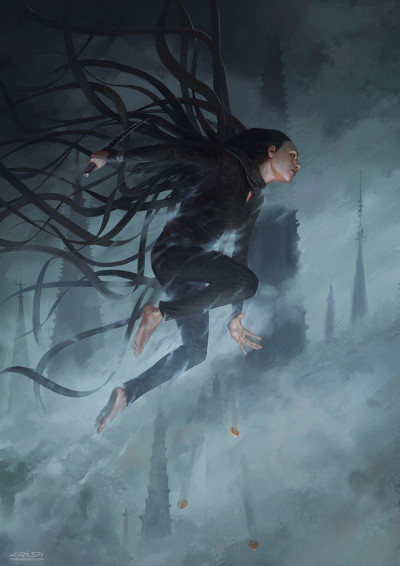
\includegraphics[width=\textwidth]
    {vin_1.png}}
  \end{figure}

  \begin{figure}[!htb]
    \center{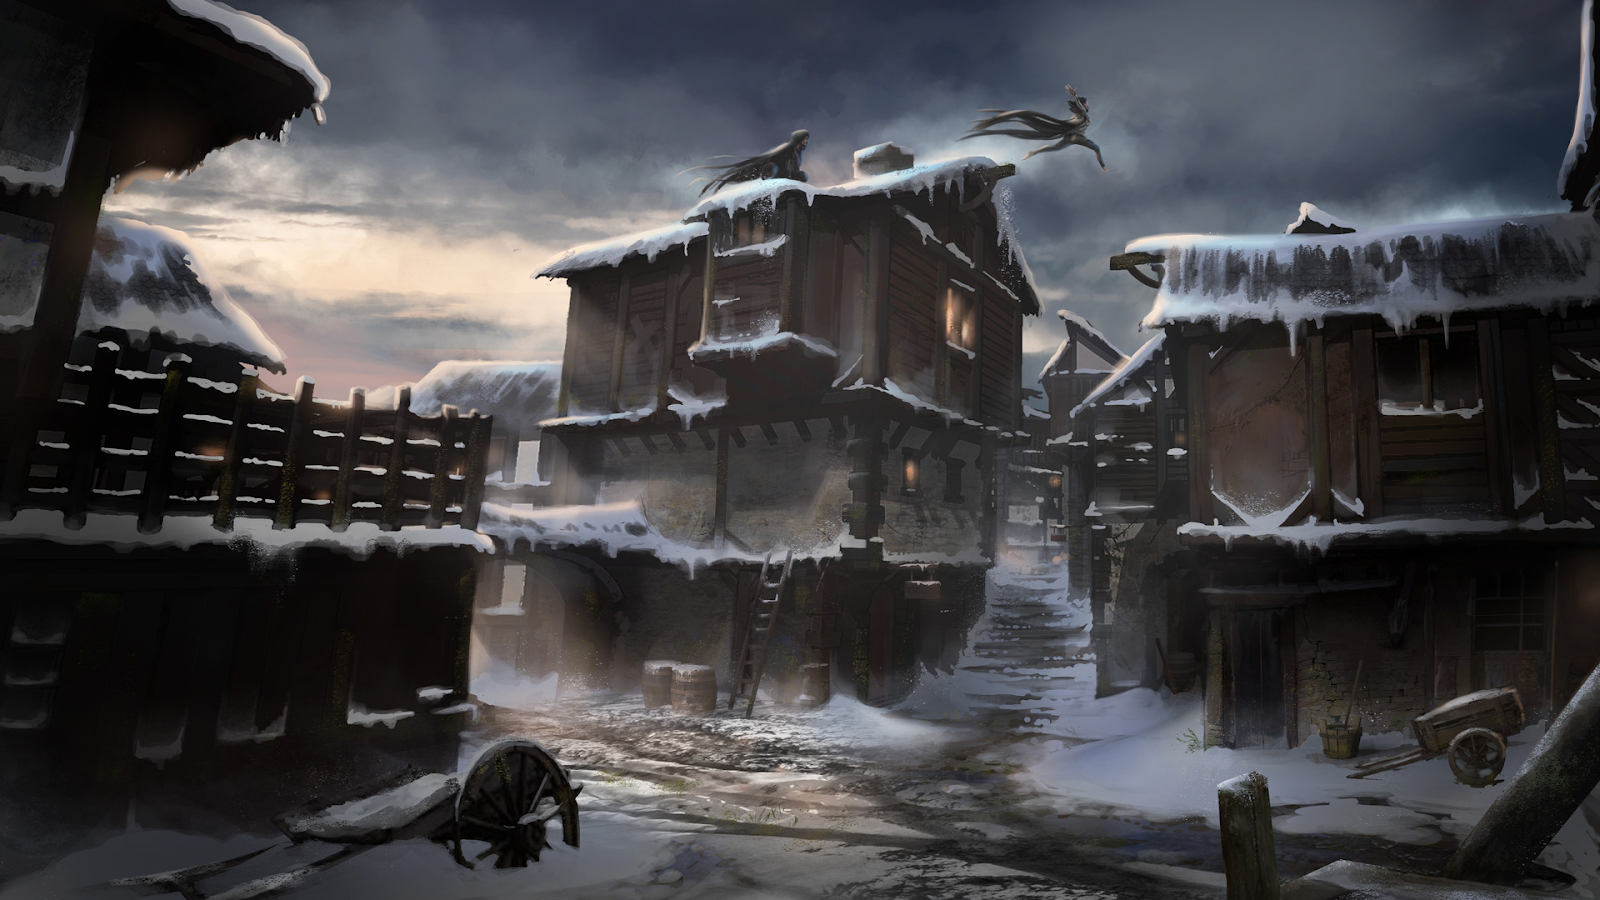
\includegraphics[width=\textwidth]
    {luthadel_0.png}}
  \end{figure}

  \begin{figure}[!htb]
    \center{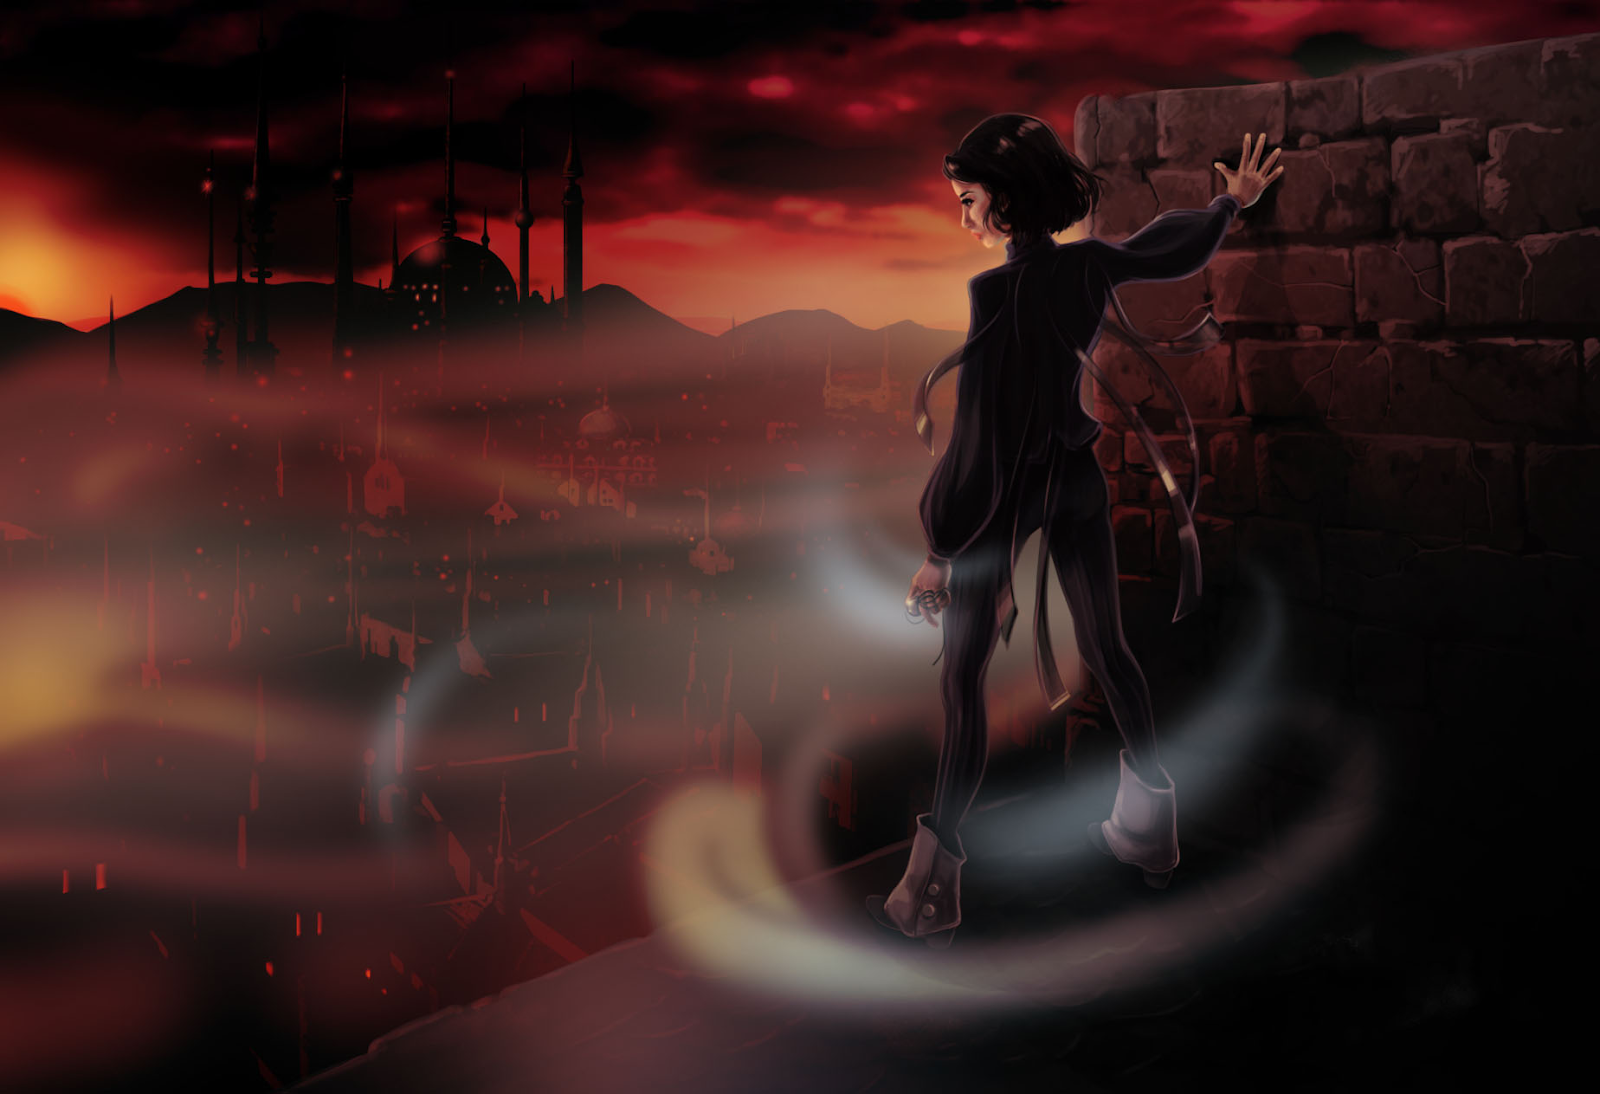
\includegraphics[width=\textwidth]
    {luthadel_1.png}}
  \end{figure}











\section{Meeting of September 25th, 2019}

\subsection{Meeting Duration}
75 Minutes

\subsection{Notes}
\subsubsection{Game Details}
\begin{description}
\item 3D characters, Platformer in a 2D view
\item Platformer
\item Singleplayer
\item Similar to Trine or This War of Mine
\item Genre: Action / Adventure platformer
\end{description}

\subsubsection{Story}
\begin{description}
\item Main character is Mistborn (NAME: YORA, THRALL, VAROK)
\item Main character loses crew member at sea, traumatic experience occurs, he snaps gets access to his powers
\item Makes it to abandoned village
\item Hears thumping sound drawing him to the Well of Ascension
\item Starts moving toward the thumping
\item When character makes it there he is confronted by Ruin - boss fight
\end{description}

\subsubsection{Enemies}
\begin{description}
\item Coinshots(ranged?)
\item Regular minions (people under Ruin’s Control)
\item Boss (Ruin)
\end{description}

\subsubsection{Mistborn Mechanics}
\begin{description}
\item Burning metals (magic system called allomancy)
\item Iron - pull metal objects toward you
\item Steel - push metal objects away from you
\item Pewter - Makes user stronger, more agile, increases endurance and healing
\item Collect metals from the environment (pots, rocks, chests)
\item Small puzzles with iron and steel (Steppable platforms that open something like doors), Levers
\item Ruin can change words (give fake hints to the player) player gambles if it is worth going there (could have traps or very powerful enemies in these areas)
\item Death takes you a checkpoint
\item Climbable walls
\item Traps (pit with spikes)
\item If you run out of metals, go back to past place where you got the resources before (once you have run out it instantly restocks)
\item Objects can drop when pulled can be used in puzzles or fighting
\item Progression issue - if someone runs out of metals, how can they complete the level.
Need to figure out what happens if player runs out of metals, (restocks supplies).
\end{description}

\subsubsection{Mistborn Setting}
\begin{description}
\item Black world, falling ash, red sun
\item Misty Environment
\end{description}

\subsubsection{Combat}
\begin{description}
\item Steel, iron fighting moving metal objects
\item Melee only available when you burn pewter
\end{description}

\subsubsection{Enemy Mechanics}
\begin{description}
\item Only attack if close enough, move towards you until it is close enough
\item Chase you to the end of the room then go back
\end{description}

\subsubsection{Sound Effects}
\begin{description}
\item Sound when player walks
\end{description}

\subsubsection{Supporting Art}
  \begin{figure}[!htb]
    \center{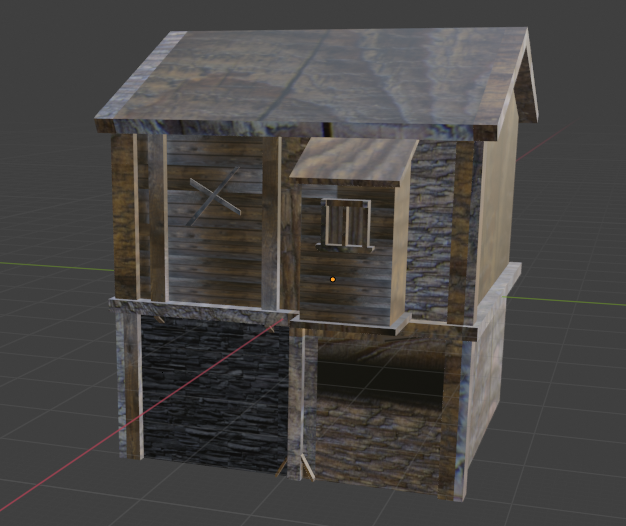
\includegraphics[width=5cm, height=5cm]
    {skaa_building_1.png}}
  \end{figure}

  \begin{figure}[!htb]
    \center{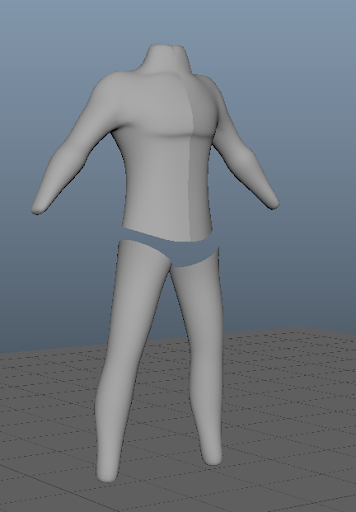
\includegraphics[width=5cm, height=5cm]
    {3D_model_body.png}}
  \end{figure}

  \begin{figure}[!htb]
    \center{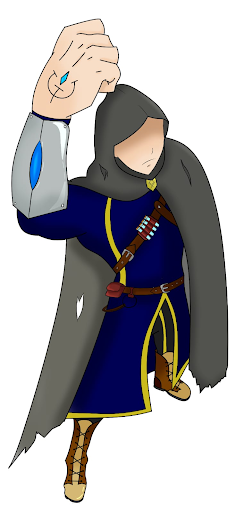
\includegraphics[width=5cm, height=5cm]
    {main_character_art_1.png}}
  \end{figure}

\newpage
 \subsubsection{Team Member Inclinations}
 \begin{description}
 \item Ayush - Animations, Player Scripting (Movement and interating with world)
 \item Luciano - Player Scripting (Abilities)
 \item Daniel - Player Scripting (Abilities)
 \item Christian - Asset Modelling, Import into Unity
 \item Samer - 
\end{description}










\section{Meeting of September 28th, 2019}

\subsection{Meeting Duration}
90 Minutes

\subsection{Notes}

\subsubsection{Summary}
Meeting was centered around building the proposal document as a team. The main character model was completed. Name of game: Mistborn - Ragnarok

\subsubsection{Proposal Presentation}
The presentation will consist of 4 parts: Introduction, Story and Setting, Mechanics, and art direction.
\begin{description}
\item Introduction - Title and tagline (introduce) - Daniel
\item Story and Setting - Explain backstory and setting, explain traumatic events leading to main character becoming mistborn (losing his crew) - Chris
\item Mechanics - Explain platformer mechanics and spend more time on the metal / potion consuming parts. Explain enemies, and how to deal with them (only fight using pewter or sneaking past) - Platforming and puzzle mechanics explained by Daniel and Metals/powers and enemies explained by Luciano
\item Related Games - Trine, INSIDE, Hollow Knight, and Claw - Ayush
\item Art Direction - How the art references resembles our setting. Explain screenshot and box art. Need a lot of images, mistborn book image, screen shots, and art - Samer
\end{description}

\subsubsection{Enemies}
\begin{description}
\item Added Koloss Enemy (Large ogre like monster)
\end{description}

\subsubsection{UI Element}
\begin{description}
\item Health bar - numeric points or hearts
\item Icons for metals carried by player
\item Simple menu to start game
\end{description}

\subsubsection{How metals/solutions should look}
\begin{description}
\item Pewter looks like power stone (purple)
\item Iron (orange)
\item Steel (silver)
\item Pewter can have a negative side effect (keep losing health while it is active)
\end{description}

\subsubsection{Supporting Art}
  \begin{figure}[!htb]
  \caption {Basic character model layout}
    \center{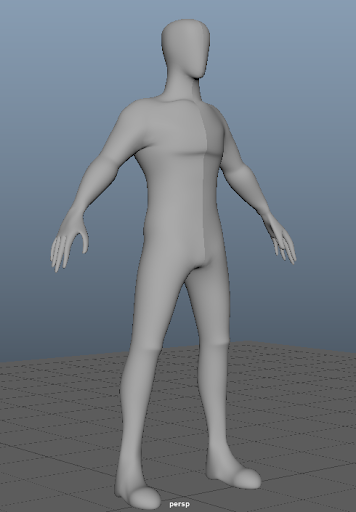
\includegraphics[width=5cm, height=5cm]
    {3D_model_body_basic.png}}
  \end{figure}

  \begin{figure}[!htb]
  \caption {Basic character with lighting}
    \center{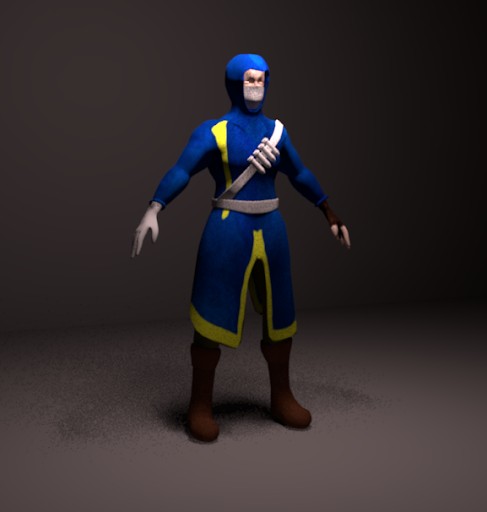
\includegraphics[width=5cm, height=5cm]
    {character_lit.png}}
  \end{figure}

  \begin{figure}[!htb]
  \caption {Basic character with lighting}
    \center{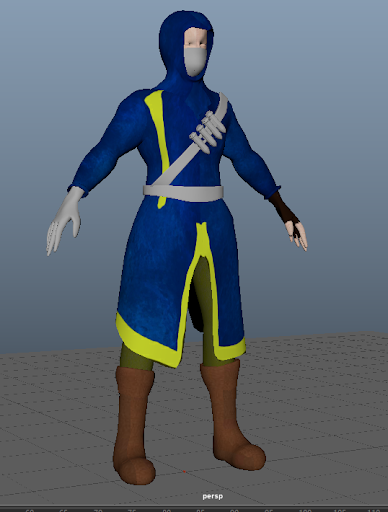
\includegraphics[width=5cm, height=5cm]
    {character_unlit.png}}
  \end{figure}

  \begin{figure}[!htb]
  \caption {Possible icon for iron solution}
    \center{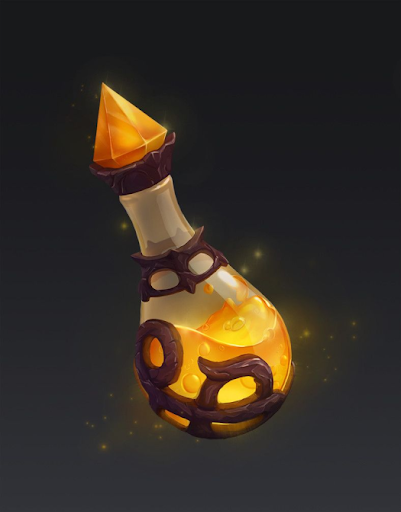
\includegraphics[width=5cm, height=5cm]
    {orange_vial.png}}
  \end{figure}

  \begin{figure}[!htb]
  \caption {Possible icon for steel solution}
    \center{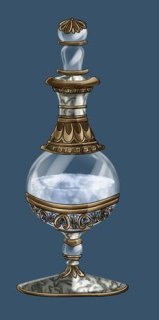
\includegraphics[width=5cm, height=5cm]
    {steel_solution.png}}
  \end{figure}

  \begin{figure}[!htb]
  \caption {Possible icon for pewter solution}
    \center{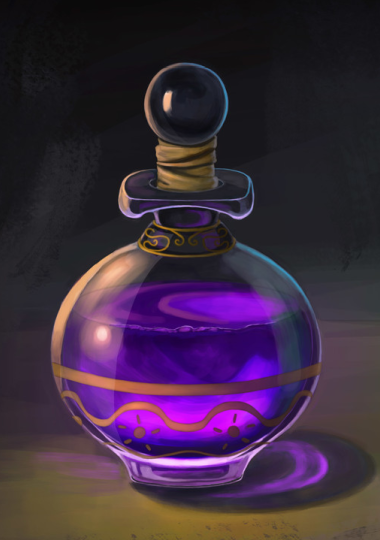
\includegraphics[width=5cm, height=5cm]
    {pewter_solution.png}}
  \end{figure}








\section{Meeting of October 2nd, 2019}

\subsection{Meeting Duration}
90 Minutes

\subsection{Notes}

\subsubsection{Summary}
Meeting was centered around polishing our proposal presentation and doing a run through of it as a team.\\*
\\*
Pull Push will work against you if you are using it on a heavy object.\\*
Once you consume, steel or iron, interactable objects will be highlighted.\\*
Consuming metals will require a 5 second animation (balancing).\\*
Pewter heals you slowly.\\*
Pewter lets you fight and increases you agility (speed and jump).\\*
Pewter will not let you one hit kill enemies.\\*
No sneaking.\\*

Breakable walls with rigid bodies\\*
Trajectory for throwing / pulling notes\\*
Do walls break? (experiment and decide)\\*

Need to think about combat system:\\*
Maybe block and attack while using pewter.\\*


Trine pulley puzzles?\\*
Cracked walls can be broken using objects with steel and iron.\\*

Can’t kill koloss by just dropping stuff on them, they are strong.\\* 

\subsubsection{Metals that exist in the world that can be interacted with}
Ship anchor\\*
Anvil (smithing)\\*
Cages for animals and humans\\*
Bell\\* 






\section{Meeting of October 9th, 2019}

\subsection{Meeting Duration}
60 Minutes

\subsection{Task Assignment}
\begin{description}
\item Ayush - Player Scripting (powers, movement)
\item Daniel - Human enemies (ai, get close enough and attack, patrolling, distance from player to engage)
\item Samer - Cutscenes (4 cutscenes (start game, level 1 to level 2, level 2 to level 3, end game))
\item Luciano - Sound Management (attack, game sounds, music)
\item Samer and Luciano - Game State Management (each cutscene is a scene, each level is a scene, saving and loading previous games, checkpoints)
\item Christian - Lay out level 1 (place assets, puzzles, objects)
\item Samer - UI (potion bar, health bar, etc.)
\item Christian - Download all the assets from the assets document on discord and place into the repo
\end{description}

Everyone makes their own branches, push there, and eventually merge assets, ui, etc. from other branches with the level layout. Team progress presentation and working game prototype with game design document due on October 31st. (Create video of game prototype)

\subsection{Boss Idea}
Boss freezes time, spawns projectiles toward you, time unfreezes and you need to dodge the projectiles (puzzle idea)




\section{Meeting of October 16th, 2019}

\subsection{Meeting Duration}
60 Minutes

\subsection{Feedback}
We went over the feedback given by other teams regarding our presentation.

Important points:
\begin{description}
\item Good balance between calm and fight moments
\item Whenever there is an eery setting force the character to walk through it. Make sure the music is not too loud so you can hear the ambient noises.
\item Could make the chests (optional ones) contain notes explaining lore for example instead of extra metal.
\end{description}

\subsection{Cutscene}
Since they were far from Ruin's influence only some of the crew got corrupted. Started killing each other, he escapes the boat after it shipwrecks. 
First - boat being destroyed
Second - Castwaway into an abandoned village
Third - Goes into an empty house searching for answers
Zoom into character's face and eyes to show determination and the character.

\subsection{Pushing Pulling Idea}
Breakable windows/walls with pushed objects. Or pull an object towards you that is behind a wall and this breaks the wall for you.

\subsection{Other}
Demo of push pull mechanics from Ayush.

\section{Meeting of October 23rd, 2019}

\subsection{Meeting Duration}
90 Minutes

\subsection{Notes}
We discussed making the jumping more responsive by adding a small delay to the time that a player can still jump off a platform to allow him to run all the way to the very edge of the platform. The rest of the session was spent working on fixing bugs regarding various aspects of level 1 including the final puzzle, issues with lever animations, and completing the layout of level 1 in preparation for the presentation the following week.

\section{Meeting of October 30th, 2019}

\subsection{Meeting Duration}
90 Minutes

\subsection{Address}
Major changes since first presentation
\begin{description}
\item We  realized that the idea of combining potion may be cool, but it didn't really make much sense to add more mechanics. 
\item It would not fit into what mechanics we currently have so
\item We will only be sticking to the 3 metals we talked about earlier.
\end{description}

Address critiques
\begin{description}
\item Important thing that was told to us in the critiques was to pay attention to the world design to capture the dark and post apocalyptic feeling in the world.
\item When we made our first level, we only concentrated on making the design.
\item If it is possible to something on top of this, we would
\item We will definitely try our best to capture this dark feeling in our second level if possible.
\end{description}

\subsection{Extra Materials}
We first planned to leave extra materials in not so obvious areas of the game, but since we choose to have a chest or a source where you could always collect metals when you run out, so instead we would leave behind anything that would explain the lore such as letters or items.

\subsection{Calm Moments}
There was one suggestion about having calm moments somewhere in the levels. We will definitely look into it, such as walking in a level which shows the character’s thoughts at that moment for immersion.

\subsection{Progress Done as Of Prototype}
Game Mechanics

\begin{description}
\item Platforming: ready
\item Ladders: ready
\item Iron and Steel abilities: ready
\item Pewter: in progress
\item Regular Enemy: ready
\item Ranged Enemy: not started
\item Combat with Pushing and Pulling: ready
\item Highlighting Interactables: not started
\item Koloss: not started
\item Boss Fight: not started
\item Level 1: ready
\item Level 2: not started
\item Boss Level: not started
\item Sound Design: in progress
\end{description}

\subsection{Other}
Now that base game mechanics are ready, we will work in parallel to design and develop level 2 and level 3, so we can speed up development.\\*\\*

An important task for us to do is: (make this one slide so they don't critique us on this).\\*\\*

Highlighting interactable objects when either steel or iron powers are active. This will make it easier for the player to find objects which they can interact with.\\*\\*

We will experiment with Unity’s shader graphs to implement this, or something simple. Plan for end product: 3 levels (one of which is boss fight). At least 1 more enemy (ranged), we might drop the idea of Koloss due to time constraints or if such an enemy doesnt fit into the game. Collectible Lore notes if it fits in time constraint. (Not a priority).

Rest of session spent practicing for the presentation.

\section{Meeting of November 6th, 2019}

\subsection{Meeting Duration}
90 Minutes

\subsection{Notes}

Discussion of points raised in the question period of the presentation (such as issues with movement of the player being clunky and too fast).

Important points discussed
\begin{description}
\item Attempt to reduce speed of player movement (without breaking the playability of the game)
\item Reduce jump length (we need to remember that it will be possible to jump further with pewter)
\item We need checkpoints in our game, especially considering the fact that the second level will be longer than the first
\item Started discussing ideas relating to the boss fight (phases, strategy to defeat, level layout)
\item We need to work on the movement of the regular enemies, their fighting is very awkward
\item Ranged Enemy: not started
\item Implementation strategy for pewter.
\end{description}

\section{Meeting of November 13th, 2019}

\subsection{Meeting Duration}
90 Minutes

\subsection{Notes}

Demo of Level 2 layout so far (initial graveyard and ideas for puzzle 1), as well as initial boss mechanics in a test scene. We also discussed the need for a pause menu in the game and also ideas for the remaining cutscenes (the ones between level 1 and level 2 and the one right before the boss).\\*

We also discussed an issue with the player jumping with the small delay at the end of platforms. Adding the delay allows the player to double jump if the spacebar is pressed twice within the delay which is totally doable. This is a game breaking issue and so we decided to remove the delay at the end. For now double jumping is actually super useful for testing since it allows us to go through levels very quickly and get to places that otherwise take a long time to get to.\\*

Dicussion of adding prompts for the player to pick up objects or interact with doors and such.
The rest of the session spent as a work session.

\section{Meeting of November 20th, 2019}

\subsection{Meeting Duration}
90 Minutes

\subsection{Notes}

The session was spent play testing the game and discussing bugs that we found.\\*

Bugs found
\begin{description}
\item Issues with player getting blocked by the chimney in level 2 puzzle 2.
\item Issues with player glitching through doors and wooden planks and ball getting stuck in ramp in puzzle 2 level 2.
\item Need for door opening at end of level 1 and animation bug on lever.
\item Opening pause menu and closing it before getting to a note causes no notes to be opened in chests (probably due to the pause key and key to close notes being the same)
\item Ranged enemy shooting at players feet (aim really poor) and coins damage player even after being shot.
\end{description}


\section{Meeting of November 27th, 2019}

\subsection{Meeting Duration}
90 Minutes

\subsection{Notes}

The session was spent play testing the game and discussing bugs that we found. Demo of teleport animations for the boss and Daniel fighting him (he is the best at fighting him and so we decided that he might be the best person to demo this part of our game since the boss fight is quite difficult). Luciano also showed us the transitions between levels and cutscenes and it seems very smooth. Sam showed us the credits and all of the cutscenes.\\*

Bugs found
\begin{description}
\item Bandit able to hit player multiple times.
\item Player able to hit boss multiple times if spam clicking.
\item Boss getting stuck in build version of game
\item Outline Shaders not showing in build version of game.
\end{description}



\end{document}